\subsection{question 2: Does “momentum” play any role in the match?}
\subsubsection{Brief Description of Our Solution}
In question 1, we develop a model to obtain momentum and then use it to measure players' performance. 
After evaluating the mechanism for obtaining momentum, we tend to disagree with the coach. Moreover, we developed an LSTM model to confirm our thought.

\subsubsection{Basic Data Analysis}
Perform statistical analysis on the momentum data obtained from the first question, and compare the momentum results of the athletes from both sides in each game. For the momentum comparison results, simply predict that the side with greater momentum will win, group each game by matchId, and finally calculate the prediction accuracy rate. Compare the final predicted winning rate with 50 percent, and the results after comparison are shown in Figure \ref{fig:PA}.
\begin{figure}
    \centering
    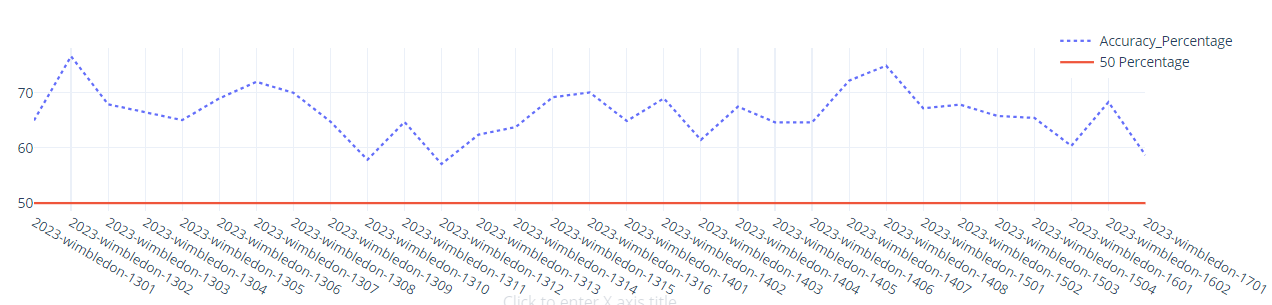
\includegraphics[width=1\linewidth]{figure/预测准确率.png}
    \caption{\centering Prediction Accuracy}
    \label{fig:PA}
\end{figure}
\subsubsection{Basic Data Analysis Results}
As can be seen from Figure \ref{fig:PA}, the accuracy rate of predicting an athlete's victory through quantified momentum exceeds 50 percent, indicating that momentum plays a role in an athlete's victory to a certain extent. Therefore, we disagree with the statement that coaching momentum is unpredictable (random).

\subsubsection{LSTM Model}
\indent LSTM (Long Short-Term Memory) is a Recurrent Neural Networks (RNN) variant designed to solve long sequence dependency problems. Recurrent neural networks can only handle close contexts but cannot get information from faraway contexts. We consider LSTM to be highly applicable to this problem for the following reasons:
\begin{itemize}
    \item \textbf{Long and Short Term Memory Mechanisms:}\ Analyzing the current tennis match should be based not only on a player's recent performance but also on the player's previous performances. The LSTM model is ideal for this problem since it consists of a " cell " memory unit, which stores and selectively forgets or passes on information to the next step. 
    \item \textbf{Advantages of RNN:}
    LSTM, a type of RNN, is often called a “black box model“due to its complex internal structure, making it challenging to understand. We can ignore the weight matrix setting process and focus solely on adjusting hyperparameters to improve the model's performance.
\end{itemize}
In this question, based on the intermediate output obtained from the AHP-TOPSIS calculation in question 1, we would like to take advantage of the above LSTM to build a model that can better predict the game's flow. Since the focus of developing the model was to confirm the correctness of our anticipated momentum, we chose to develop a base model that uses the intermediate output from momentum as input and the result of the score as output.

\subsubsection{LSTM Experiment Result}
We first initialized the model using the stochastic method and did not train it, as expected, the model had an average accuracy of 0.5. Random momentum doesn't affect the game's outcome. We aim to improve accuracy by training the model to show that predicted momentum impacts the match. \par


\begin{table}[b!]  
\caption{\centering LSTM Basic Params}% [] control the position of table
    \centering
    % \renewcommand{\arraystretch}{1.5}
    \begin{tabular}{c c}            % main part of table: {} control alignment(l,c,r)
        \toprule 
        Param & Value \\
        \midrule
        Optimizer & Adam \\
        Learning Rate & 0.001 \\
        Loss Function & BCEWithLogitsLoss \\
        Early Stop & 10 \\
        Batch Size & 32 \\
        \bottomrule
    \end{tabular}
    \vspace{10pt}
    \vspace{-5pt}
    \label{tab:lstm1}
\end{table}
Through some basic experiments, we first determined some model parameters, recorded in Table \ref{tab:lstm1}. 
Next, we experimented with several parameters whose effect on the model could not be determined. 
\begin{figure}[bt!]
    \centering
    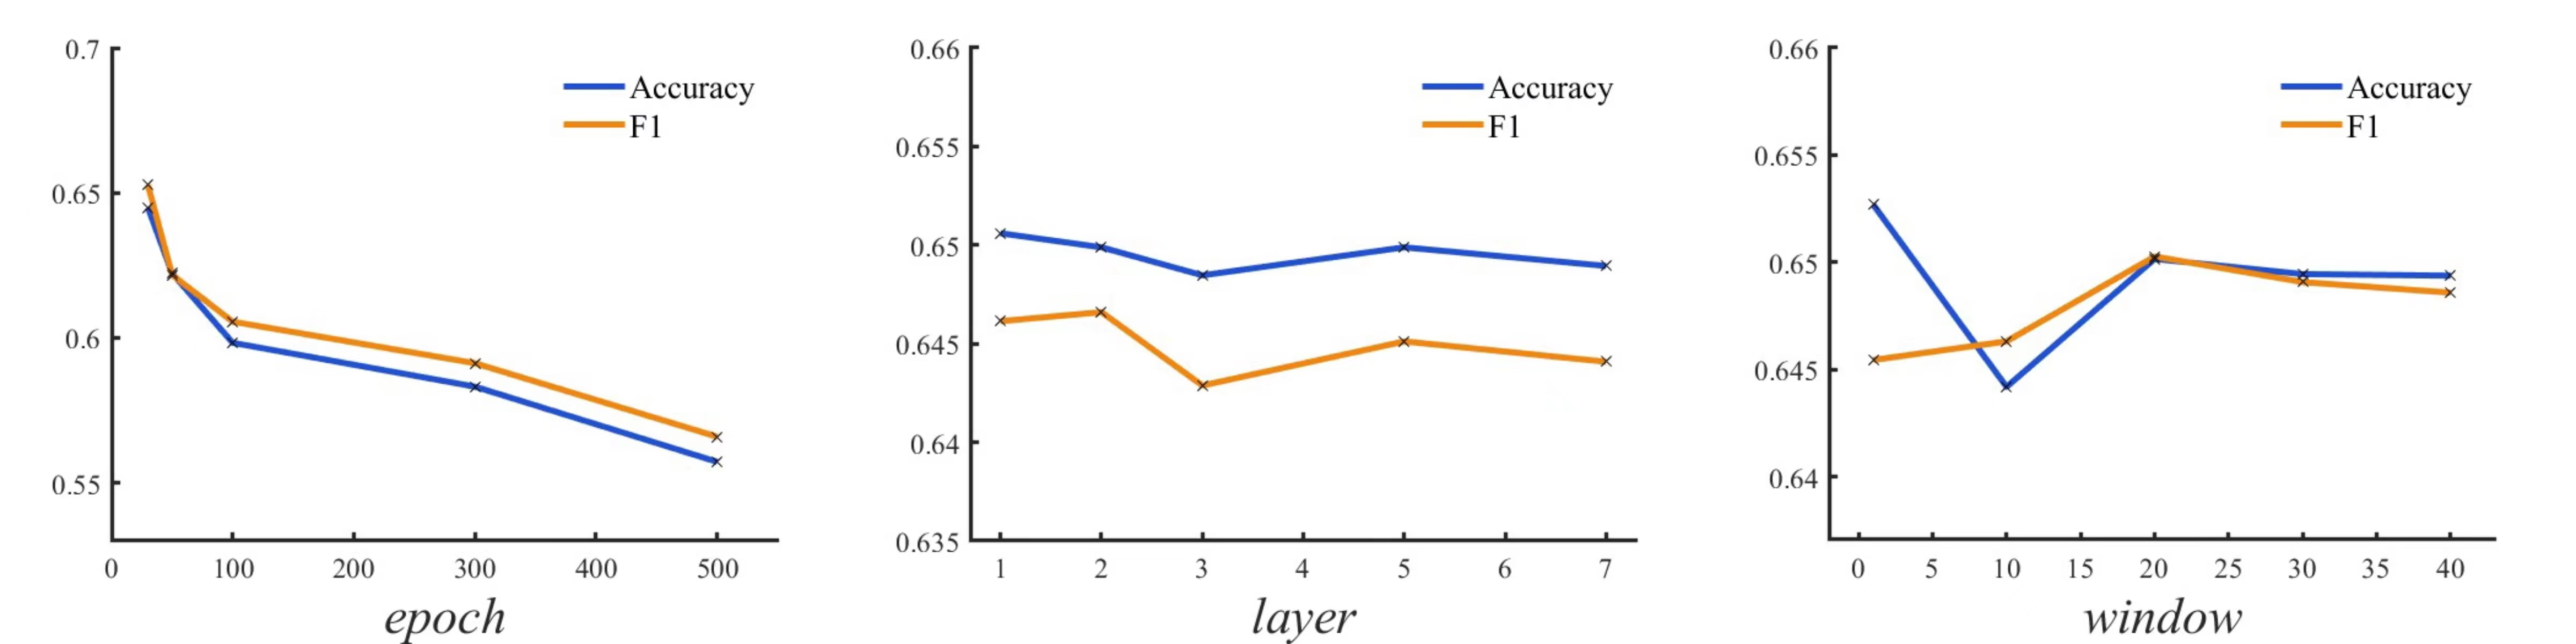
\includegraphics[width=1\linewidth]{figure/lstm1.jpg}
    \caption{\centering LSTM Parameters}
    \label{fig:lstm1}
\end{figure}
The result of our experiment is displayed in Figure \ref{fig:lstm1}. \par
During our experiments, we faced the biggest challenge in training machine models due to the lack of data and the difficulty in data augmentation. \par 
The experimental results suggest that increasing the hidden size to create a larger model by adding more parameters can lead to overfitting. Although these larger models can be trained well for multiple epochs, resulting in a low training loss, they tend to perform poorly on the test set. \par
We decided to use a small model for prediction, even though we faced difficulty achieving a satisfactory loss during the training process. However, the negligible difference between the results of the test set and the training set eventually led to a higher accuracy in the outcome.\par
In the end, we obtained an average accuracy of 0.65, which we believe is sufficient to demonstrate the correlation between momentum and game, given the varied nature of the games. \par


\subsubsection{Discussion}
\textbf{Layers of LSTM: }
After concluding our experiment, we initially attempted to explain the lack of significance of the LAYER. We considered factors such as vanishing or exploding gradients versus data complexity, but none seemed to be the right explanation. Ultimately, we determined that adding more layers increases the number of parameters. As previously discussed, this particular problem is not well-suited for large models.\par
\textbf{Window Size: }
Window Size refers to the number of scores the model will consider forward for the current situation. In the given problem, the window size plays a crucial role as it determines the memory extent that LSTM considers. According to our analysis, the model seems to struggle in making use of data from past units due to the inputs being summarized data. However, in the later developed LSTM model, we observed that the window size effect increased by inputting raw data. \par